\documentclass[11pt]{article}
\usepackage[utf8]{inputenc}

%%%%%%%%%%%%%%%%%%%%%%%%%%%%%%%%%%%%%%%%%%%%%%%%%%%%%%%%%%%%%%%%
% PACKAGES, FORMATTING, LISTING, AND OTHER GRAPHICAL ELEMENTS  %
%%%%%%%%%%%%%%%%%%%%%%%%%%%%%%%%%%%%%%%%%%%%%%%%%%%%%%%%%%%%%%%%

\usepackage{amsmath,amssymb}
\usepackage[T1]{fontenc} % font encoding
\usepackage{graphicx} % for figures
\usepackage{float} % for figures
\usepackage{indentfirst} % indent first paragraph of section
\usepackage{soul,xcolor} % for colors
\usepackage{xkcdcolors} % colors from XKCD color survey
\usepackage{mathtools} % for boxed equations within \align
\usepackage{sectsty} % adjust section headers
\usepackage{fancyhdr} % page headers
\usepackage{titling} % reference title,author,date (in fancyhdr page header)
\usepackage{breqn} % automatically line wrap long Eqs.
\usepackage{pdfpages} % for \includepdf
\usepackage{pdflscape} % landscape 
\usepackage{mdframed} % for framed environment
\usepackage{listings} % for code blocks
\usepackage{inconsolata} % better monospace font
\usepackage{matlab-prettifier} % Better MATLAB listing highlighting
\usepackage[letterpaper, total={6.5in, 9in}]{geometry} % set paper and margin size
\usepackage{empheq} % multiline boxed equations, etc.
\usepackage{hyperref}
\usepackage{dsfont}	% gives you \mathds{} font
% \usepackage{enumerate} % custom enumerate numbering (or lettering in this case)
\usepackage[shortlabels]{enumitem} % more enumerate options
\usepackage{svg} % use inkscape to import svgs
\usepackage{bm} % bold symbols
\usepackage[parfill]{parskip} % replace indentation with paragraph spacing
\usepackage{dsfont} % gives you \mathds{} font

% hyperbolic trig inverse functions
\DeclareMathOperator{\sech}{sech}
\DeclareMathOperator{\csch}{csch}
\DeclareMathOperator{\arcsec}{arcsec}
\DeclareMathOperator{\arccot}{arcCot}
\DeclareMathOperator{\arccsc}{arcCsc}
\DeclareMathOperator{\arccosh}{arcCosh}
\DeclareMathOperator{\arcsinh}{arcsinh}
\DeclareMathOperator{\arctanh}{arctanh}
\DeclareMathOperator{\arcsech}{arcsech}
\DeclareMathOperator{\arccsch}{arcCsch}
\DeclareMathOperator{\arccoth}{arcCoth} 

% add page headers
\pagestyle{fancy}
\fancyhf{}
\fancyhead[LE,LO]{\thetitle}
\fancyhead[RE,RO]{\theauthor}
\fancyfoot[CE,CO]{\thepage}

% adjust section header font size
\sectionfont{\fontsize{20}{15}\selectfont}
\subsectionfont{\fontsize{14}{15}\selectfont}

% vertical table spacing
\renewcommand{\arraystretch}{1.5}

% right-side cases
% \newenvironment{rcases}
%     {\left.\begin{aligned}}
%     {\end{aligned}\right\rbrace}

% Multi-line \fbox
\newcommand\multilineBox[1]{
\noindent
\fbox{
	\parbox{0.97\linewidth}
		{#1}
	}
}

% number just one equation in an un-numbered align* environment
\newcommand\numberthis{\addtocounter{equation}{1}\tag{\theequation}}

%%%%%%%%%%%%%%%%%%%%%%%%%%%%%%%%%%%%%%%%%%%%%%%%%%%%%%%%%%%%%%%%

% set listings font to inconsolata
\DeclareFixedFont{\ttb}{T1}{txtt}{bx}{n}{9} % for bold
\DeclareFixedFont{\ttm}{T1}{txtt}{m}{n}{9}  % for normal

% general listings environment
\lstnewenvironment{code}
{\lstset{
    frame=single,
    % backgroundcolor=\color{xkcdPale},
    basicstyle=\fontfamily{pcr}\selectfont\tiny
    }}
{}

% MATLAB listings environment
\lstnewenvironment{MATLAB}
{\lstset{
    style=Matlab-editor,
    frame=single,
    % backgroundcolor=\color{xkcdPale},
    basicstyle=\fontfamily{pcr}\selectfont\tiny
    }}
{}

% Python style for listings
\newcommand\pythonstyle{\lstset{
    language=Python,
    basicstyle=\ttm,
    morekeywords={self},              % Add keywords here
    keywordstyle=\ttb\color{xkcdGreen},
    morekeywords=[2]{
        array,
        pi,
        zeros,
        max,
        sin,
        cos,
        linspace,
        size,
        plot,
        xlabel,
        title,
        legend,
        show,
        concatenate,
        logspace,
        exp,
        ylabel,
        savefig,
        grid,
        figure,
        axes
    },
    keywordstyle = [2]{\color{xkcdBrightBlue}},
    emph={__init__},                  % Custom highlighting
    emphstyle=\ttb\color{xkcdRed},    % Custom highlighting style
    stringstyle=\color{xkcdGreen},
    backgroundcolor=\color{xkcdPale},
    numberstyle=\color{xkcdGrey},
}}

% Python listings environment
\lstnewenvironment{python}[1][]
{\pythonstyle \lstset{#1}}
{}

% Python listings for external files
\newcommand\pythonexternal[2][]
{{\pythonstyle \lstinputlisting[#1]{#2}}}

% Python listings inline
\newcommand\pythoninline[1]{{\pythonstyle \lstinline!#1!}}


%%%%%%%%%%%%%%%%%%%%%%%%%%%%%%%%%%%%%%%%%%%%%%%%%%%%%%%%%%%%%%%%
% MATHEMATICAL SHORTCUTS                                       %
%%%%%%%%%%%%%%%%%%%%%%%%%%%%%%%%%%%%%%%%%%%%%%%%%%%%%%%%%%%%%%%%

% real and imaginary components
\renewcommand{\Re}{\operatorname{Re}}
\renewcommand{\Im}{\operatorname{Im}}

% Fourier transforms
\newcommand\fourier[1]{\frac{1}{\sqrt{2\pi}} \int_{-\infty}^\infty #1 e^{-i\omega x} \textrm{d}x}
\newcommand\inverseFourier[1]{\frac{1}{\sqrt{2\pi}} \int_{-\infty}^\infty #1 e^{i\omega x} \textrm{d}\omega}

% derivatives
\newcommand{\ppf}[2]{\frac{\partial #1}{\partial #2}}
\newcommand{\pppf}[3]{\frac{\partial^2 #1}{\partial #2 \partial #3}}
\newcommand{\ddf}[2]{\frac{\text{d} #1}{\text{d} #2}}
\newcommand{\DDf}[2]{\frac{\text{D} #1}{\text{D} #2}}

% norms
\newcommand\norm[1]{\lVert#1\rVert}

% statistical operators
\newcommand{\prob}{\operatorname{P}}
\newcommand{\expectation}{\operatorname{E}}
\newcommand{\variance}{\operatorname{Var}}
\newcommand{\stddev}{\operatorname{SD}}

% statistical distributions
\newcommand{\bernoulli}{\operatorname{Bernoulli}}
\newcommand{\binomial}{\operatorname{Binomial}}
\newcommand{\poisson}{\operatorname{Poisson}}
\newcommand{\normal}{\operatorname{Normal}}

%%%%%%%%%%%%%%%%%%%%%%%%%%%%%%%%%%%%%%%%%%%%%%%%%%%%%%%%%%%%%%%%
% COMMONLY USED COPYPASTAS
%%%%%%%%%%%%%%%%%%%%%%%%%%%%%%%%%%%%%%%%%%%%%%%%%%%%%%%%%%%%%%%%

% CODE BLOCK

% \begin{MATLAB}[caption={MATLAB script},label={code:p1}]
% for i = 1:n
%     disp('string')
% end
% \end{MATLAB}
% Code block \ref{code:p1}



% MULTIPLE EQUATIONS BOXED

% \begin{empheq}[box=\fbox]{align}
% \end{empheq}



% ENUMERTATE WITH a) instead of 1.

% \begin{enumerate}[label=\alph*)]
% \end{enumerate}
% 'Problem' sections
% \renewcommand{\thesection}{Part \arabic{section}}
\renewcommand{\thesubsection}{\arabic{section}.\alph{subsection}}
% \renewcommand{\thesubsection}{\arabic{subsection}}

\title{ENGR 510 Intro to Machine Learning Homework}
\author{Anthony Su}
\date{November 5, 2024}

\begin{document}
\thispagestyle{plain}
\maketitle


%%%%%%%%%%%%%%%%%%%%%%%%%%%%%%%%%%%%%%%%%%%%%%%%%%%%%%%%%%%%%%%%
% PART 1
%%%%%%%%%%%%%%%%%%%%%%%%%%%%%%%%%%%%%%%%%%%%%%%%%%%%%%%%%%%%%%%%
\section{}

\setcounter{subsection}{1}  % skip 1.1

\subsection{}  % 1.2 -------------------------------------------
\begin{figure}[H]
    \centering
    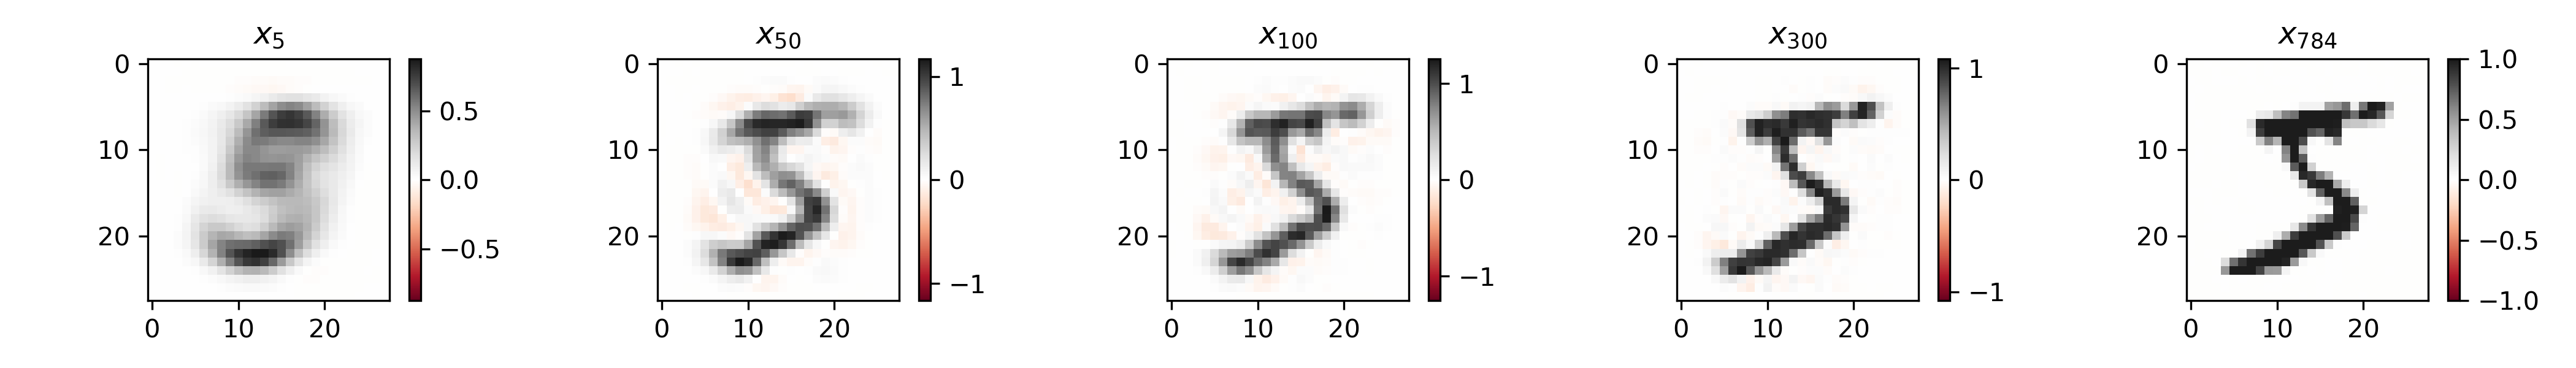
\includegraphics[width=\textwidth]{1.2fig1.png}
    \caption{PCA Reconstructions of the first image in the dataset using
        $r=[5, 50, 100, 300]$.}
    \label{fig_1.2_1}
\end{figure}

Note that in Fig. \ref{fig_1.2_1}, $x_{784}$ is the true image. Also, note that
the mean of the data was re-introduced when generating this plot.

\subsection{}  % 1.3 -------------------------------------------
\begin{figure}[H]
    \centering
    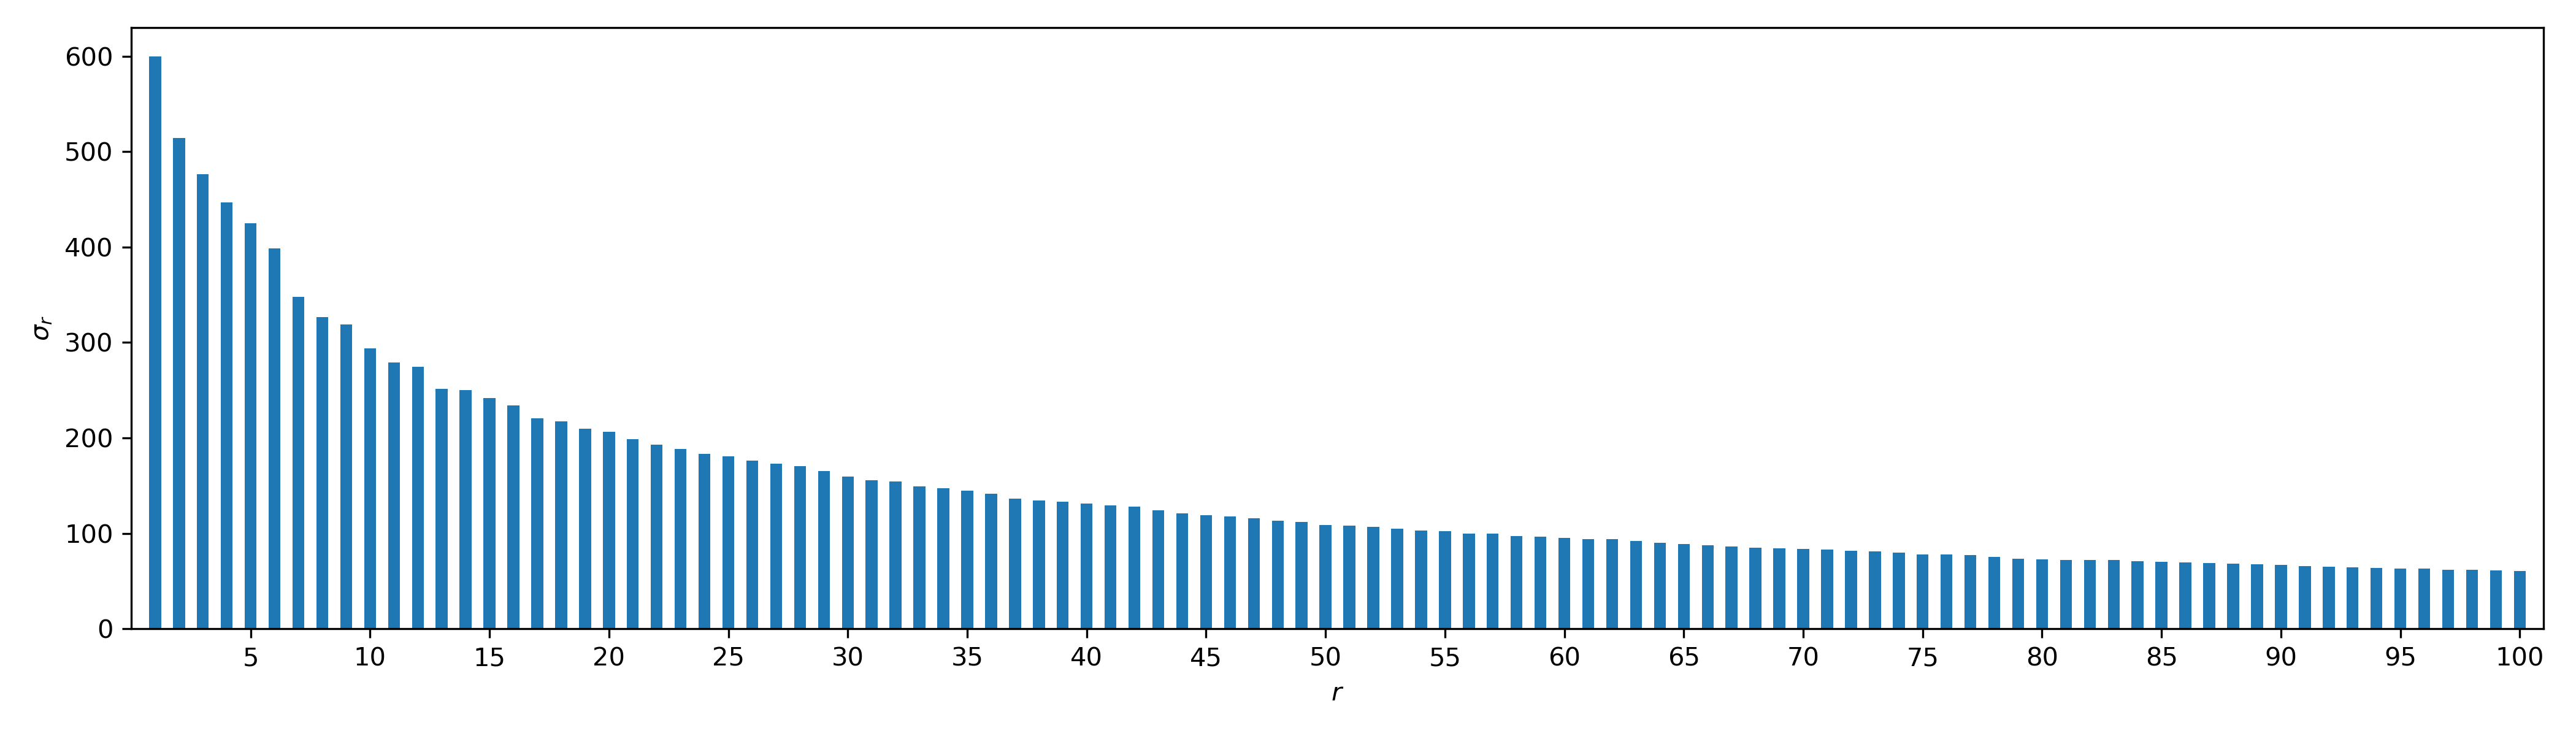
\includegraphics[width=\textwidth]{1.3fig1.png}
    \caption{First 100 singular values}
    \label{fig_1.3_1}
\end{figure}

\subsection{}  % 1.4 -------------------------------------------
\begin{figure}[H]
    \centering
    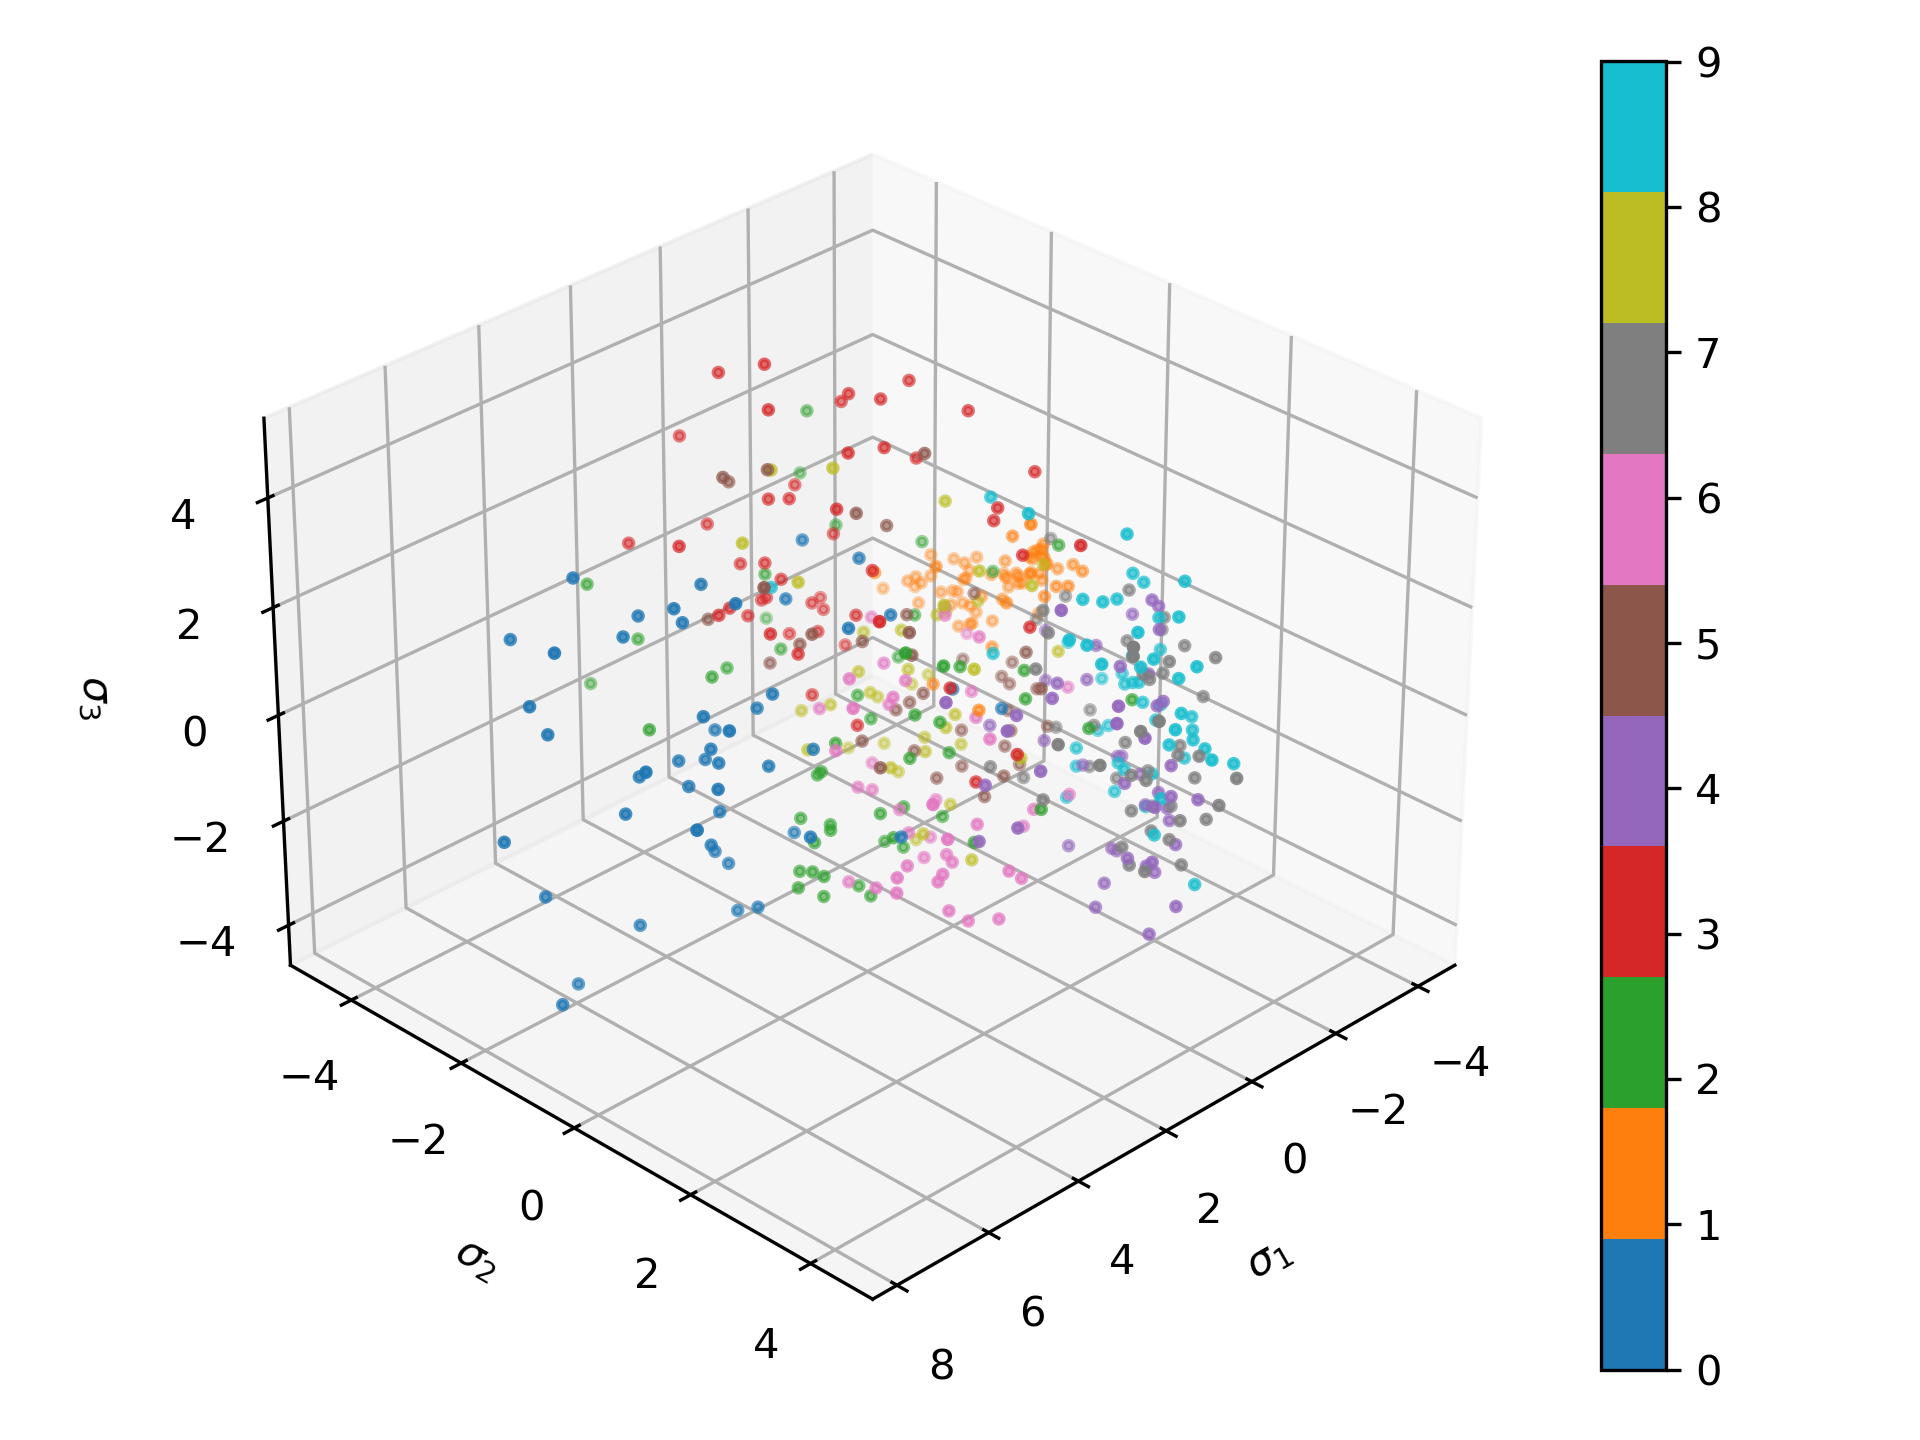
\includegraphics[width=0.6\textwidth]{1.4fig1.png}
    \caption{500 data points in the $r=350$ PCA space projected into the first three components}
    \label{fig_1.4_1}
\end{figure}
The digits 4 and 9 appear difficult to separate as they lie in the same region
and have significant overlap. The digits 0 and 9 appear easy to separate as they
lie in separate regfions with minimal overlap.

%%%%%%%%%%%%%%%%%%%%%%%%%%%%%%%%%%%%%%%%%%%%%%%%%%%%%%%%%%%%%%%%
% PART 2
%%%%%%%%%%%%%%%%%%%%%%%%%%%%%%%%%%%%%%%%%%%%%%%%%%%%%%%%%%%%%%%%
\section{}

\setcounter{subsection}{4}  % skip 1.1, 1.2, 1.3, and 1.4

\subsection{}  % 2.5 -------------------------------------------
\begin{figure}[H]
    \centering
    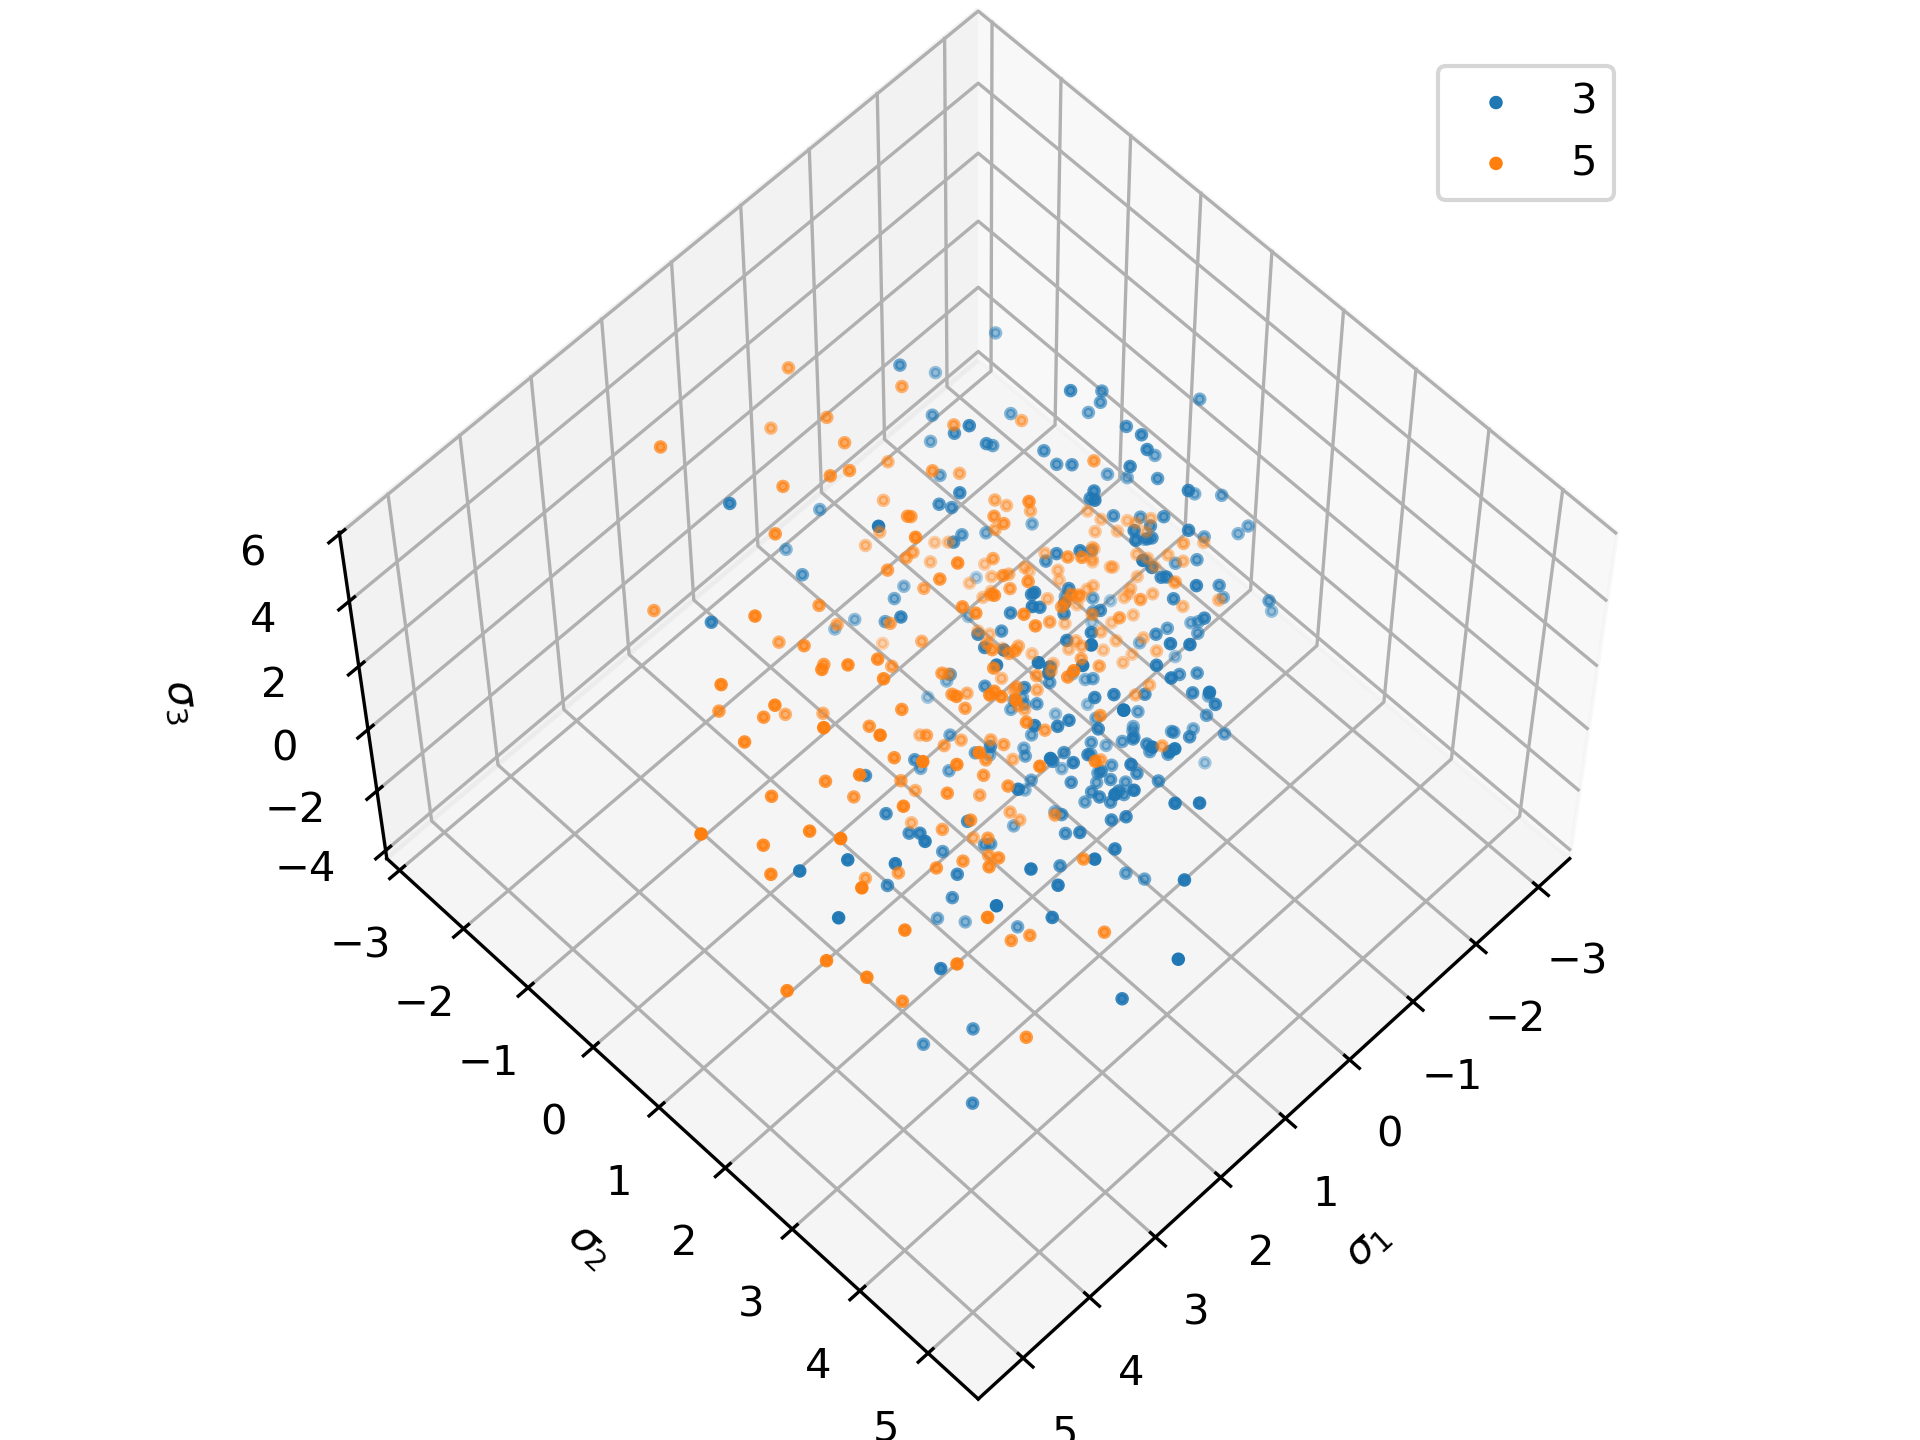
\includegraphics[width=0.6\textwidth]{2.5fig1.png}
    \caption{Hardest digit pair for LDA: 3 and 5}
    \label{fig_2.5_1}
\end{figure}
\begin{figure}[H]
    \centering
    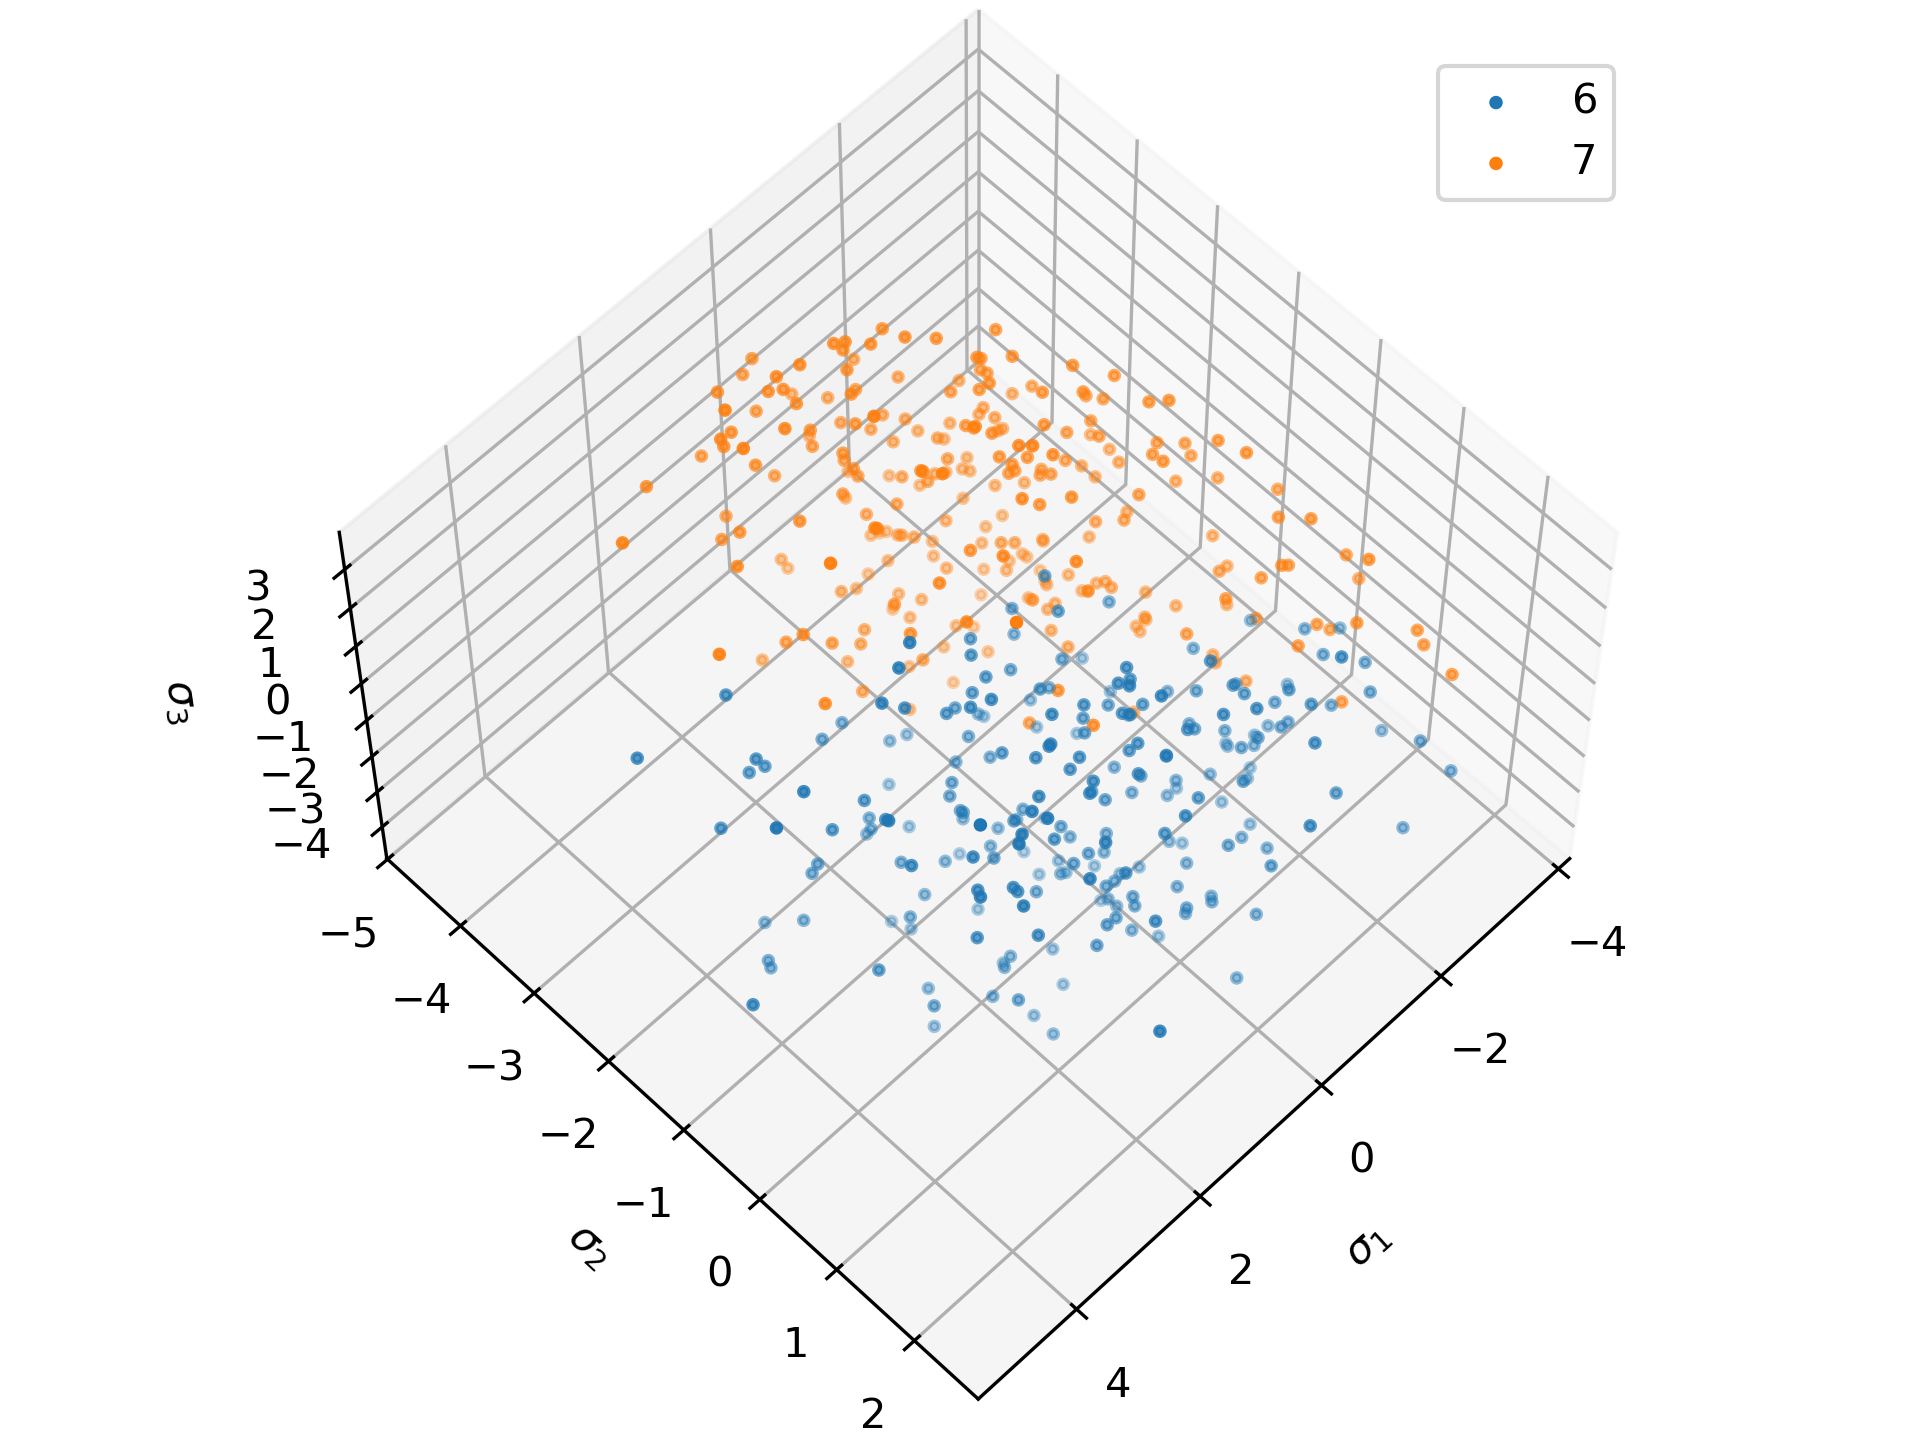
\includegraphics[width=0.6\textwidth]{2.5fig2.png}
    \caption{Easiest digit pair for LDA: 6 and 7}
    \label{fig_2.5_2}
\end{figure}

In Fig. \ref{fig_2.5_1}, there is significant overlap between the regions
occupied by the two digits. In contrast, in Fig. \ref{fig_2.5_2}, there is
a relatively clean separation betwen the regions occupied by the two digits.

\end{document}